\documentclass[11pt,a4paper]{report}

% --------------------------------------------------
% Packages
% --------------------------------------------------
\usepackage[a4paper,margin=1in]{geometry}
\usepackage{graphicx}
\usepackage{float}
\usepackage{booktabs}
\usepackage{array}
\usepackage{tabularx}
\usepackage{longtable}
\usepackage{xcolor}
\usepackage{hyperref}
\usepackage{fancyhdr}
\usepackage{titlesec}
\usepackage{setspace}
\usepackage{enumitem}
\usepackage{caption}
\usepackage{listings}
\usepackage{tikz}
\usetikzlibrary{positioning}
\usepackage{tcolorbox}
\usepackage{needspace}

% --------------------------------------------------
% Colors
% --------------------------------------------------
\definecolor{primary}{HTML}{17365D}
\definecolor{secondary}{HTML}{2F75B5}
\definecolor{lightblue}{HTML}{EAF2F8}
\definecolor{lightgray}{HTML}{F4F6F7}
\definecolor{darkgray}{HTML}{444444}
\definecolor{critical}{HTML}{922B21}
\definecolor{high}{HTML}{C0392B}
\definecolor{medium}{HTML}{D68910}
\definecolor{low}{HTML}{2874A6}

% --------------------------------------------------
% Hyperlinks
% --------------------------------------------------
\hypersetup{
    colorlinks=true,
    linkcolor=primary,
    urlcolor=secondary,
    citecolor=primary,
    pdftitle={OWASP Juice Shop VAPT Report},
    pdfauthor={Routhu Mohan}
}

% --------------------------------------------------
% Page Style
% --------------------------------------------------
\pagestyle{fancy}
\fancyhf{}
\fancyhead[L]{\textbf{OWASP Juice Shop VAPT}}
\fancyhead[R]{Security Assessment Report}
\fancyfoot[C]{\thepage}

\setlength{\headheight}{14pt}

% --------------------------------------------------
% Spacing
% --------------------------------------------------
\setstretch{1.2}

% --------------------------------------------------
% Chapter Style
% --------------------------------------------------
\titleformat{\chapter}
    {\normalfont\Huge\bfseries\color{primary}}
    {\thechapter}
    {1em}
    {}

\titleformat{\section}
    {\normalfont\Large\bfseries\color{primary}}
    {\thesection}
    {1em}
    {}

\titleformat{\subsection}
    {\normalfont\large\bfseries\color{secondary}}
    {\thesubsection}
    {1em}
    {}

% --------------------------------------------------
% Tables
% --------------------------------------------------
\renewcommand{\arraystretch}{1.25}

% --------------------------------------------------
% Captions
% --------------------------------------------------
\captionsetup{
    font=small,
    labelfont=bf
}

% --------------------------------------------------
% Code / Command Style
% --------------------------------------------------
\lstset{
    backgroundcolor=\color{lightgray},
    basicstyle=\ttfamily\small,
    frame=single,
    breaklines=true,
    columns=fullflexible
}

% --------------------------------------------------
% Lists
% --------------------------------------------------
\setlist[itemize]{itemsep=3pt,topsep=4pt}
\setlist[enumerate]{itemsep=3pt,topsep=4pt}

% --------------------------------------------------
% Document
% --------------------------------------------------
\begin{document}

% ==================================================
% COVER PAGE
% ==================================================

\begin{titlepage}
    \centering

    \vspace*{1.5cm}

    {\Huge\bfseries\color{primary}
    OWASP Juice Shop VAPT Report\par}

    \vspace{0.5cm}

    {\Large
    Vulnerability Assessment and Penetration Testing\par}

    \vspace{1.2cm}

    \rule{\textwidth}{1pt}

    \vspace{0.4cm}

    {\large\bfseries Security Assessment Report\par}

    \vspace{0.4cm}

    \rule{\textwidth}{1pt}

    \vfill

    {\large\textbf{Prepared By}\par}

    \vspace{0.25cm}

    {\Large Routhu Mohan\par}

    \vspace{0.8cm}

    \begin{tabular}{rl}
        \textbf{Target:} & OWASP Juice Shop \\
        \textbf{Environment:} & Localhost \\
        \textbf{Assessment Type:} & VAPT
    \end{tabular}

    \vfill

    {\large September 2026 \par}

\end{titlepage}

% ==================================================
% TABLE OF CONTENTS
% ==================================================

\pagenumbering{roman}

\tableofcontents

\clearpage

% ==================================================
% MAIN REPORT
% ==================================================

\pagenumbering{arabic}

\chapter{Executive Summary}
\label{chap:executive-summary}
\subsection*{Assessment Overview}

The assessment began with the definition of the testing scope,
objectives, rules of engagement, and target environment. Reconnaissance
activities were then performed to identify application functionality,
endpoints, parameters, and other accessible components.

Automated security testing was performed using tools such as OWASP
ZAP and FFUF, while SQLMap was used where appropriate for SQL
Injection assessment. The identified potential vulnerabilities were
then manually verified using techniques including crafted HTTP
requests and Burp Suite.

Only vulnerabilities that were successfully validated and supported
by appropriate evidence were included as confirmed findings in this
report.

\subsection*{Confirmed Findings}

A total of eight vulnerabilities were confirmed during the
assessment.

\begin{table}[H]
\centering
\renewcommand{\arraystretch}{1.25}
\begin{tabular}{|l|p{6cm}|l|}
\hline
\textbf{Finding ID} & \textbf{Vulnerability} & \textbf{Severity} \\
\hline
BAC & Broken Access Control -- Privilege Escalation via Registration
& Critical \\
\hline
IDOR & Insecure Direct Object Reference -- Unauthorized Basket Access
& Medium \\
\hline
AUTH & Weak Password Recovery & Critical \\
\hline
SQLI-01 & SQL Injection -- Authentication Bypass & Critical \\
\hline
SQLI-02 & SQL Injection -- Product Search and Data Extraction
& High \\
\hline
XSS & Reflected Cross-Site Scripting -- Search Parameter & Medium \\
\hline
CSRF & Cross-Site Request Forgery -- Profile Update & Medium \\
\hline
OR & Open Redirect -- Unvalidated Redirect Parameter & Medium \\
\hline
\end{tabular}
\caption{Summary of confirmed vulnerabilities}
\end{table}

\subsection*{Severity Distribution}

The confirmed findings consist of three Critical-severity findings,
one High-severity finding, and four Medium-severity findings.

\begin{itemize}
    \item \textbf{Critical:} 3 findings
    \item \textbf{High:} 1 finding
    \item \textbf{Medium:} 4 findings
    \item \textbf{Low:} 0 findings
\end{itemize}

The Critical findings include Broken Access Control, SQL Injection --
Authentication Bypass, and Weak Password Recovery. The single
High-severity finding is SQL Injection -- Product Search and Data
Extraction. Reflected XSS, IDOR, CSRF, and Open Redirect were
classified as Medium severity based on the demonstrated impact and
exploitation conditions.

\subsection*{Key Security Observations}

The assessment identified weaknesses across several important
application security controls.

The SQL Injection findings demonstrate insufficient protection of
user-controlled input used by database-related functionality. The
login functionality was found to be susceptible to authentication
bypass, while the product search functionality was found to allow
unauthorized database interaction under the tested conditions.

The Broken Access Control finding demonstrates a weakness in
server-side authorization and privilege assignment. The Weak Password
Recovery finding demonstrates that an attacker can take over the
affected account without knowledge of the original password. If the
same weakness affected a privileged account, it could potentially lead
to unauthorized administrative access.

The remaining findings affect resource authorization, client-side
script
execution, state-changing requests, and redirect handling.
Together, these findings demonstrate that security controls should be
strengthened across multiple areas of the application.

\subsection*{Business and Security Impact}

The confirmed vulnerabilities may affect the confidentiality,
integrity, and security of application resources depending on the
specific vulnerability and exploitation conditions.

The Critical and High severity findings require particular attention
because they affect authentication, authorization, account recovery,
and database interaction.

If similar weaknesses existed in a production application handling
real user information, successful exploitation could result in
unauthorized access, modification of application resources, exposure
of data, account compromise, or execution of attacker-controlled
content.

\subsection*{Recommended Actions}

The identified vulnerabilities should be addressed according to their
severity and associated risk.

Priority should be given to implementing parameterized database
queries, enforcing server-side authorization and role assignment,
strengthening password recovery controls, implementing object-level
authorization checks, and applying appropriate output encoding and
request protection.

Additional controls should include secure redirect validation,
appropriate security headers, least-privilege access, server-side
input validation, and security monitoring.

After remediation, all confirmed findings should be retested using
the original proof-of-concept techniques and additional relevant test
cases to verify that the vulnerabilities have been effectively
addressed.

\subsection*{Report Scope}

This report documents the testing activities, identified
vulnerabilities, supporting evidence, impact assessment, and
recommended remediation measures within the defined assessment scope.

The findings and conclusions presented in this report are based on
the testing performed against the specified OWASP Juice Shop
environment during this engagement.

\chapter{Introduction}
\label{chap:introduction}
This report presents the results of a Vulnerability Assessment and
Penetration Testing (VAPT) assessment conducted against a locally
hosted OWASP Juice Shop application. OWASP Juice Shop is a deliberately
vulnerable web application that provides a controlled environment for
identifying and understanding common web application security
weaknesses.

The assessment was performed in a controlled environment with the
objective of examining the security of the application from an
attacker-oriented perspective. The testing process combined automated
security tools with manual testing and verification techniques.

The assessment was organized into a structured sequence of activities,
beginning with planning and scoping, followed by reconnaissance,
vulnerability scanning and assessment, and manual verification and
proof-of-concept testing. The results from these activities were used
to identify potential security weaknesses and select findings for
further manual analysis and validation.

The assessment confirmed eight security vulnerabilities covering
multiple security areas, including Broken Access Control, Insecure
Direct Object Reference (IDOR), Weak Password Recovery, SQL Injection,
Reflected Cross-Site Scripting (XSS), Cross-Site Request Forgery
(CSRF), and Open Redirect. Evidence was collected during testing to
support each confirmed finding and provide a clear record of the
assessment activities.

The confirmed findings consisted of three Critical-severity findings,
one High-severity finding, and four Medium-severity findings. The
Critical findings included Broken Access Control, SQL Injection --
Authentication Bypass, and Weak Password Recovery. The single
High-severity finding was SQL Injection -- Product Search and Data
Extraction, while Reflected XSS, IDOR, CSRF, and Open Redirect were
classified as Medium severity.

The remainder of this report presents the assessment objectives,
scope, methodology, tools, phase-wise testing activities, confirmed
vulnerabilities, risk assessment, remediation recommendations,
retesting activities, and supporting evidence.

% ==================================================
% CHAPTER 3 -- ASSESSMENT APPROACH
% ==================================================

\chapter{Assessment Approach}
\label{chap:assessment-approach}

\section{Project Objectives}
This section defines the objectives of the Vulnerability Assessment
and Penetration Testing (VAPT) engagement conducted against the
locally hosted OWASP Juice Shop application.

The primary objective of the assessment was to identify and manually
validate security vulnerabilities that could affect the
confidentiality, integrity, and availability of application
resources and user functionality.

The specific objectives of the assessment were:

\begin{itemize}

    \item \textbf{Identify security vulnerabilities} in the OWASP
    Juice Shop web application through systematic security testing.

    \item \textbf{Perform reconnaissance} to identify accessible
    endpoints, application functionality, parameters, and other
    relevant attack surfaces.

    \item \textbf{Perform automated vulnerability assessment} using
    appropriate security testing tools to identify potential
    vulnerabilities and security weaknesses.

    \item \textbf{Perform manual security testing} to verify
    vulnerabilities identified through automated scanning and to
    identify weaknesses that may not be detected automatically.

    \item \textbf{Validate identified vulnerabilities} using
    controlled proof-of-concept techniques without causing
    unnecessary disruption to the application.

    \item \textbf{Assess the security impact} of each confirmed
    vulnerability based on the demonstrated exploitation and affected
    application functionality.

    \item \textbf{Collect supporting evidence} such as HTTP
    requests and responses, scanner results, screenshots, and
    proof-of-concept results for each confirmed finding.

    \item \textbf{Classify confirmed vulnerabilities} according to
    their severity and relevant security classification frameworks,
    including OWASP and CWE where applicable.

    \item \textbf{Provide remediation recommendations} for the
    confirmed vulnerabilities to help strengthen the application's
    security controls.

    \item \textbf{Define retesting requirements} to verify that
    vulnerabilities are effectively addressed after remediation.

\end{itemize}

The assessment was conducted within the defined scope and controlled
testing environment. Testing activities were focused on identifying
and validating security weaknesses in the target application rather
than causing permanent modification or disruption to the system.

\section{Scope and Rules of Engagement}
This section defines the target, boundaries, and rules followed during
the Vulnerability Assessment and Penetration Testing (VAPT) engagement.
The assessment was performed in a controlled local laboratory
environment.

\subsection{Assessment Scope}

The assessment was performed against a locally hosted instance of the
OWASP Juice Shop application. The target and testing boundaries were
defined before the assessment began.

\begin{table}[!htb]
\centering
\begin{tabularx}{\textwidth}{>{\bfseries}p{0.32\textwidth} X}
\toprule
Assessment Item & Details \\
\midrule
Target Application & OWASP Juice Shop \\
Target URL & \texttt{http://127.0.0.1:3000} \\
Environment & Local laboratory environment \\
Assessment Type & Web Application VAPT \\
Testing Approach & Manual and automated testing \\
\bottomrule
\end{tabularx}
\caption{Assessment target and environment}
\end{table}

\subsection{In-Scope Components}

The following parts of the application were included in the
assessment:

\begin{itemize}
    \item OWASP Juice Shop web application
    \item Application pages, routes, and endpoints
    \item REST API endpoints
    \item Authentication and session mechanisms
    \item User-controlled input fields and parameters
    \item Application access-control mechanisms
    \item HTTP communication between the client and server
    \item Security-related application configurations
\end{itemize}

\subsection{Out-of-Scope Components}

The following components and activities were not included in the
assessment:

\begin{itemize}
    \item External websites and third-party services
    \item Other devices or systems on the local network
    \item Exploitation of the host operating system
    \item Denial-of-Service (DoS) testing
    \item Any system outside the defined OWASP Juice Shop laboratory
    environment
\end{itemize}

\subsection{Rules of Engagement}

The following rules were followed during the assessment:

\begin{itemize}
    \item Testing was restricted to the locally hosted OWASP Juice
    Shop instance.

    \item Testing activities were limited to the defined assessment
    scope.

    \item No testing was performed against real-world or unauthorized
    systems.

    \item Denial-of-Service testing was excluded from the assessment.

    \item Vulnerabilities identified during testing were documented
    with appropriate supporting evidence.

    \item Testing was performed in a controlled laboratory environment
    for educational and cybersecurity training purposes.
\end{itemize}

\subsection{Assessment Authorization}

The OWASP Juice Shop application was hosted locally as an
intentionally vulnerable application for security testing and
educational purposes.

All activities documented in this report were therefore limited to
the defined local laboratory environment and the specified target
application.

\section{VAPT Methodology}
The assessment followed a structured Vulnerability Assessment and Penetration
Testing (VAPT) methodology. The methodology was designed to move from
initial planning and reconnaissance to vulnerability identification,
validation, documentation, and remediation.

\begin{figure}[!htb]
\centering
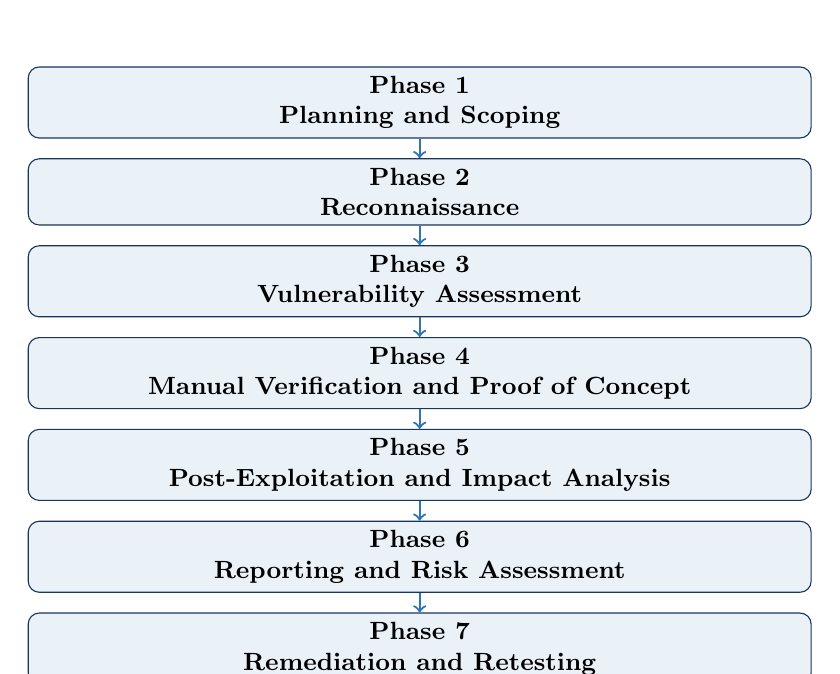
\begin{tikzpicture}[
    node distance=0.25cm,
    every node/.style={
        font=\small\bfseries,
        align=center
    },
    phase/.style={
        rectangle,
        rounded corners,
        draw=primary,
        fill=lightblue,
        minimum width=0.82\textwidth,
        minimum height=0.65cm
    },
    arrow/.style={
        ->,
        thick,
        color=secondary
    }
]

\node[phase] (p1) {Phase 1\\Planning and Scoping};
\node[phase, below=of p1] (p2) {Phase 2\\Reconnaissance};
\node[phase, below=of p2] (p3) {Phase 3\\Vulnerability Assessment};
\node[phase, below=of p3] (p4) {Phase 4\\Manual Verification and Proof of Concept};
\node[phase, below=of p4] (p5) {Phase 5\\Post-Exploitation and Impact Analysis};
\node[phase, below=of p5] (p6) {Phase 6\\Reporting and Risk Assessment};
\node[phase, below=of p6] (p7) {Phase 7\\Remediation and Retesting};

\draw[arrow] (p1) -- (p2);
\draw[arrow] (p2) -- (p3);
\draw[arrow] (p3) -- (p4);
\draw[arrow] (p4) -- (p5);
\draw[arrow] (p5) -- (p6);
\draw[arrow] (p6) -- (p7);

\end{tikzpicture}
\caption{VAPT assessment methodology}
\end{figure}

Each phase shown above is documented as its own chapter later in this
report: Phase 1 in Chapter~\ref{chap:phase1}, Phase 2 in
Chapter~\ref{chap:phase2}, Phase 3 in Chapter~\ref{chap:phase3},
Phase 4 in Chapter~\ref{chap:phase4}, Phase 5 in
Chapter~\ref{chap:phase5}, Phase 6 in Chapter~\ref{chap:phase6}, and
Phase 7 in Chapter~\ref{chap:phase7}.

\section{Tools and Technologies}
The assessment used a combination of manual and automated security
testing tools. Each tool was selected based on the specific activity
it supported during reconnaissance, vulnerability assessment, and
manual validation. Detailed usage of each tool, along with evidence,
is documented within the relevant phase chapters later in this
report.

\begin{table}[!htb]
\small
\centering
\begin{tabularx}{\textwidth}{>{\bfseries}p{0.20\textwidth}
                                X
                                p{0.24\textwidth}}
\toprule
Tool & Primary Purpose & Assessment Activity \\
\midrule

Browser &
Manual exploration of application pages, functions, and accessible
resources &
Reconnaissance \\

Nmap &
Port, service, and basic network discovery &
Reconnaissance \\

Wappalyzer &
Identification of technologies, frameworks, and application
components &
Technology Identification \\

robots.txt Review &
Manual review of the application's robots.txt file to identify
disclosed or restricted paths &
Reconnaissance \\

Burp Suite &
Interception and analysis of HTTP requests and responses, including
headers, cookies, methods, and parameters &
Manual Testing and Validation \\

OWASP ZAP &
Application crawling, Spider and AJAX Spider discovery, passive
scanning, and active security scanning &
Reconnaissance and Vulnerability Assessment \\

ffuf &
Discovery of directories, endpoints, and accessible application
paths &
Endpoint Discovery \\

SQLMap &
Automated testing and verification of SQL Injection vulnerabilities &
Vulnerability Assessment \\

\bottomrule
\end{tabularx}
\caption{Security tools used during the assessment}
\label{tab:recon-tools}
\end{table}

% ==================================================
% CHAPTER 4 -- PHASE 1
% ==================================================

\chapter{Phase 1 -- Planning and Scoping}
\label{chap:phase1}
This phase established the foundation for the OWASP Juice Shop VAPT
assessment. The full target definition, scope, and rules of
engagement are defined in Chapter~3 (Assessment Approach,
Section~3.2) and were confirmed and locked in during this phase
before the technical assessment began.

\section{Phase Objectives}

The main purpose of the planning and scoping phase was to establish a
clear and controlled assessment environment. The objectives of this
phase were to:

\begin{itemize}
    \item Define the target application and assessment environment.
    \item Establish the scope of the security assessment.
    \item Identify the testing approach and assessment boundaries.
    \item Define the rules of engagement for the assessment.
    \item Establish the methodology to be followed during the
    subsequent phases.
\end{itemize}

\section{Assessment Methodology}

The project was organized into the following seven VAPT phases, as
detailed in Chapter~3, Section~3.3:

\begin{enumerate}
    \item Planning and Scoping
    \item Reconnaissance
    \item Vulnerability Assessment
    \item Manual Verification and Proof of Concept
    \item Post-Exploitation and Impact Analysis
    \item Reporting and Risk Assessment
    \item Remediation and Retesting
\end{enumerate}

The planning phase established the foundation for the reconnaissance,
vulnerability assessment, and manual verification activities that
followed.

\section{Expected Deliverables}

The planned assessment deliverables included:

\begin{itemize}
    \item Reconnaissance findings
    \item Vulnerability scanning and assessment results
    \item Confirmed vulnerability findings
    \item Proof-of-concept evidence
    \item Risk and impact analysis
    \item Remediation recommendations
    \item Final VAPT report
\end{itemize}

\section{Phase 1 Summary}

Table~\ref{tab:phase1-summary} summarizes the outcomes confirmed
during this phase before the assessment progressed to
reconnaissance.

\begin{table}[H]
\centering
\begin{tabularx}{\textwidth}{>{\bfseries}p{0.35\textwidth} X}
\toprule
Planning Item & Outcome \\
\midrule
Target Definition & Confirmed (Section~3.2) \\
Assessment Scope & Confirmed (Section~3.2) \\
Rules of Engagement & Confirmed (Section~3.2) \\
Assessment Methodology & Confirmed (Section~3.3) \\
Authorization \& Environment & Confirmed -- local, isolated
laboratory instance \\
\bottomrule
\end{tabularx}
\caption{Phase 1 planning outcomes}
\label{tab:phase1-summary}
\end{table}

\section{Phase Completion}

Phase 1 was completed after the project scope, target, objectives,
testing boundaries, and methodology had been confirmed. The
assessment then progressed to the reconnaissance phase.

% ==================================================
% CHAPTER 5 -- PHASE 2
% ==================================================

\chapter{Phase 2 -- Reconnaissance}
\label{chap:phase2}
The reconnaissance phase focused on understanding the target application,
identifying exposed services and technologies, and mapping the observable
application attack surface before vulnerability assessment activities began.

\section{Objective}

The objective of this phase was to identify the target application, discover
its exposed network and application-level components, identify the technologies
in use, and collect information that could support the subsequent vulnerability
assessment.

The reconnaissance activities included technology identification, review of
accessible application information, port and service discovery, directory and
endpoint discovery, HTTP traffic analysis, and automated application crawling.
The tools used during this phase are listed in Table~\ref{tab:recon-tools}
in Chapter~3, Section~3.4.

\section{Target Identification}

The target application was confirmed to be accessible through the local
browser at \texttt{http://127.0.0.1:3000}. The application loaded successfully
and was available for subsequent reconnaissance and security testing.

\begin{figure}[H]
    \centering
    
\includegraphics[width=0.90\textwidth]
    {evidence/phase2/images-proved/01-target-application.png}
    \caption{OWASP Juice Shop target application accessible at
    \texttt{http://127.0.0.1:3000}.}
    \label{fig:recon-target}
\end{figure}

\section{Port and Service Discovery}

Nmap was used to identify open ports and gather basic service information
from the target host. The scan identified port \texttt{3000/tcp} as open,
which was consistent with the locally hosted web application.

\begin{figure}[H]
    \centering
    
\includegraphics[width=0.90\textwidth]
    {evidence/phase2/images-proved/02-nmap-port-scan.png}
    \caption{Nmap port scan results showing port \texttt{3000/tcp} open.}
    \label{fig:recon-nmap-ports}
\end{figure}

A service-detection scan was also performed to gather additional information
about the service exposed on the identified port.

\begin{figure}[H]
    \centering
    
\includegraphics[width=0.90\textwidth]
    {evidence/phase2/images-proved/03-nmap-service-detection.png}
    \caption{Nmap service detection results for the identified web service.}
    \label{fig:recon-nmap-service}
\end{figure}

\section{Technology Identification}

Wappalyzer was used to identify technologies and frameworks associated with
the target application. The results provided information about the client-side
frameworks, libraries, content delivery services, and programming technologies
observed during reconnaissance.

\begin{figure}[H]
    \centering
    
\includegraphics[width=0.85\textwidth]
    {evidence/phase2/images-proved/04-wappalyzer-technologies.png}
    \caption{Wappalyzer technology identification results.}
    \label{fig:recon-wappalyzer}
\end{figure}

\section{\texttt{robots.txt} Analysis}

The application's \texttt{robots.txt} file was directly accessed and reviewed
for path information that could reveal additional application resources.

The file contained a disallowed \texttt{/ftp} path, providing an additional
resource for reconnaissance and subsequent security testing.

\begin{figure}[H]
    \centering
    
\includegraphics[width=0.90\textwidth]
    {evidence/phase2/images-proved/05-robots-txt.png}
    \caption{Contents of the application's \texttt{robots.txt} file.}
    \label{fig:recon-robots}
\end{figure}

\section{HTTP Request and Response Analysis}

Burp Suite was used as an intercepting proxy to observe HTTP communication
between the browser and the target application.

The captured traffic provided visibility into the HTTP methods, request
headers, cookies, target paths, and server responses. A successful
\texttt{HTTP/1.1 200 OK} response was observed for the captured request.

\begin{figure}[H]
    \centering
    
\includegraphics[width=0.95\textwidth]
    {evidence/phase2/images-proved/06-burp-http-request-response.jpeg}
    \caption{Burp Suite HTTP request and response captured during reconnaissance.}
    \label{fig:recon-burp}
\end{figure}

\section{Directory and Endpoint Discovery}

ffuf was used to perform active directory and endpoint discovery against the
target application. A commonly used web-content wordlist was used to identify
accessible paths that were not necessarily visible through normal application
navigation.

The scan identified multiple accessible paths, including examples such as
\texttt{/api}, \texttt{/ftp}, \texttt{/rest}, \texttt{/assets}, and
\texttt{/robots.txt}.

\begin{figure}[H]
    \centering
    
\includegraphics[width=0.90\textwidth]
    {evidence/phase2/images-proved/07-ffuf-directory-discovery.png}
    \caption{ffuf directory and endpoint discovery results.}
    \label{fig:recon-ffuf}
\end{figure}

\section{OWASP ZAP Spider}

The OWASP ZAP Spider was used to automatically crawl the target application
and identify reachable resources and links.

The completed Spider scan reported:

\begin{itemize}
    \item \textbf{URLs Found:} 398
    \item \textbf{Nodes Added:} 255
\end{itemize}

The crawl identified a number of application resources and REST-style
endpoints that expanded the observable attack surface.

\begin{figure}[H]
    \centering
    
\includegraphics[width=0.95\textwidth]
    {evidence/phase2/images-proved/08-zap-spider-results.png}
    \caption{OWASP ZAP Spider results showing 398 URLs found and 255 nodes added.}
    \label{fig:recon-zap-spider}
\end{figure}

\section{OWASP ZAP AJAX Spider}

The OWASP ZAP AJAX Spider was additionally used to crawl the application through
browser-based navigation and identify resources and routes associated with
client-side application behavior.

The completed AJAX Spider scan reported:

\begin{itemize}
    \item \textbf{URLs Crawled:} 383
\end{itemize}

The AJAX crawl provided additional visibility into dynamically requested
resources and JavaScript-driven application behavior.

\begin{figure}[H]
    \centering
    
\includegraphics[width=0.95\textwidth]
    {evidence/phase2/images-proved/09-zap-ajax-spider-results.png}
    \caption{OWASP ZAP AJAX Spider results showing 383 URLs crawled.}
    \label{fig:recon-zap-ajax}
\end{figure}

\section{Reconnaissance Summary}

The reconnaissance activities established an initial view of the application's
observable attack surface.

The target was confirmed to be accessible at
\texttt{http://127.0.0.1:3000}, and Nmap identified port
\texttt{3000/tcp} as open. Wappalyzer identified multiple technologies and
frameworks associated with the application.

The review of \texttt{robots.txt} revealed the \texttt{/ftp} path, while ffuf
identified additional application paths and resources. Burp Suite provided
visibility into HTTP request and response behavior. OWASP ZAP further expanded
the observable application map through both traditional and AJAX-based
crawling.

The information collected during this phase was used to guide vulnerability
scanning and assessment activities in Phase 3 and manual verification and
proof-of-concept testing in Phase 4.

\begin{table}[H]
\centering
\begin{tabularx}{\textwidth}{>{\bfseries}p{0.38\textwidth} X}
\toprule
Metric & Result \\
\midrule
Target &
\texttt{http://127.0.0.1:3000} \\

Open Port Identified &
\texttt{3000/tcp} \\

ffuf Discovery &
Multiple accessible paths identified \\

ZAP Spider &
398 URLs / 255 nodes \\

ZAP AJAX Spider &
383 URLs crawled \\

\texttt{robots.txt} Observation &
\texttt{/ftp} path disclosed \\

HTTP Analysis &
Successful \texttt{HTTP/1.1 200 OK} response observed \\
\bottomrule
\end{tabularx}
\caption{Reconnaissance phase summary}
\label{tab:recon-summary}
\end{table}

\section{Phase 3 Preparation}

The reconnaissance results established the initial attack surface that was
used to guide Phase 3 vulnerability scanning and assessment activities.

A complete de-duplicated endpoint inventory is not included in this section
until the raw ffuf, ZAP Spider, and AJAX Spider outputs have been consolidated.
This avoids presenting a partial endpoint list as a complete inventory.

% ==================================================
% CHAPTER 6 -- PHASE 3
% ==================================================

\chapter{Phase 3 -- Vulnerability Assessment}
\label{chap:phase3}
\section{Objective}

Phase 3 was performed to identify possible security weaknesses in
the OWASP Juice Shop application using automated scanning.

The main tool used in this phase was OWASP ZAP. The scan was used to
find potential vulnerabilities that required further testing.

The alerts generated during this phase were treated as potential
findings. They were not considered confirmed vulnerabilities until
they were manually tested in Phase 4.

\section{Scanning Methodology}

The following scanning activities were performed using OWASP ZAP:

\begin{enumerate}

    \item \textbf{Spider Scan} -- The traditional Spider was used to
    crawl the application and discover available pages, links, and
    endpoints.

    \item \textbf{AJAX Spider} -- The AJAX Spider was used because
    Juice Shop is a JavaScript-based application. It helped discover
    additional pages and content that may not be found by the
    traditional Spider.

    \item \textbf{Passive Scan} -- ZAP analyzed the traffic generated
    during browsing and crawling. This helped identify common
    security issues without actively attacking the application.

    \item \textbf{Active Scan} -- ZAP actively tested the discovered
    application endpoints for possible vulnerabilities, including
    SQL Injection, Cross-Site Scripting, and other web security
    issues.

    \item \textbf{Alert Review} -- The alerts generated by ZAP were
    reviewed and compared with the application's actual behavior.
    Findings that required further testing were carried forward to
    Phase 4 for manual validation.

\end{enumerate}

\section{ZAP Scan Evidence}

The following evidence shows the OWASP ZAP alerts identified during
the scanning process for the two findings that were flagged by
automated scanning: SQL Injection (SQLI-02) and Open Redirect (OR).

\begin{figure}[H]
    \centering
    
\includegraphics[width=0.8\textwidth]
    {evidence/phase3/zap/sqli02-01-zap-alert-detection.png}
    \caption{OWASP ZAP identifying a possible SQL Injection vulnerability
    in the product search parameter}
    \label{fig:zap-sqli02}
\end{figure}

\begin{figure}[H]
    \centering
    
\includegraphics[width=0.8\textwidth]
    {evidence/phase3/zap/openredirect-01-zap-alert-detection.png}
    \caption{OWASP ZAP identifying a possible Open Redirect
    vulnerability in the redirect parameter}
    \label{fig:zap-or}
\end{figure}

Both alerts shown above were treated as potential vulnerabilities.
Further testing was performed in Phase 4 using Burp Suite (and
SQLMap for SQLI-02) to confirm each issue and determine its actual
impact. Full exploitation details are provided in
Sections~7.4 and~7.7.

\section{Scan Results}

The OWASP ZAP scan generated a total of 18 alerts.

The alerts were reviewed before deciding which issues required
detailed manual testing. An alert from an automated scanner does not
always mean that a real vulnerability exists. Therefore, the findings
were manually tested before being included as confirmed
vulnerabilities in this report.

\begin{table}[H]
\centering
\begin{tabular}{|l|l|}
\hline
\textbf{Scan Result} & \textbf{Count} \\
\hline
Total ZAP Alerts & 18 \\
\hline
Findings Selected for Phase 4 Validation & 2 \\
\hline
Other Alerts Not Carried Forward & 16 \\
\hline
\end{tabular}
\caption{Summary of OWASP ZAP scan results}
\end{table}

\section{Findings Selected for Manual Validation}

The following two findings were identified through automated
scanning and selected for further testing and evidence collection in
Phase 4:

\begin{table}[H]
\centering
\begin{tabular}{|l|p{8cm}|}
\hline
\textbf{Finding ID} & \textbf{Vulnerability} \\
\hline
SQLI-02 & SQL Injection -- Product Search Parameter \\
\hline
OR & Open Redirect -- Unvalidated Redirect Parameter \\
\hline
\end{tabular}
\caption{Findings selected for Phase 4 validation (ZAP-detected)}
\end{table}

The remaining confirmed findings -- BAC, IDOR, AUTH,
SQLI-01 (Authentication Bypass through Login), XSS, and CSRF --
were not flagged by the OWASP ZAP automated scan and were instead
identified through manual testing during Phase 4, as documented in
their respective finding sections.

\section{Phase 3 to Phase 4}

Phase 3 was mainly used for automated discovery. The alerts provided
an initial indication of possible security weaknesses for two of the
eight confirmed findings.

In Phase 4, both the ZAP-flagged findings and the additional
manually-identified findings were tested and confirmed using Burp
Suite and other appropriate tools. Evidence was collected to prove
whether each issue was actually exploitable and to understand its
security impact.

Therefore, the report follows this process:

\begin{center}
\textbf{Automated Scanning / Manual Discovery}
$\rightarrow$
\textbf{Alert Review}
$\rightarrow$
\textbf{Manual Validation}
$\rightarrow$
\textbf{Evidence Collection}
$\rightarrow$
\textbf{Confirmed Finding}
\end{center}

\section{Note}

The detailed technical information and exploitation evidence for the
confirmed vulnerabilities are provided in the Phase 4 finding
chapters.

The purpose of Phase 3 is to document how potential vulnerabilities
were discovered, while Phase 4 provides the detailed proof and impact
of the confirmed vulnerabilities.

% ==================================================
% CHAPTER 7 -- PHASE 4: MANUAL VERIFICATION AND PROOF OF CONCEPT
% ==================================================

\chapter{Phase 4 -- Manual Verification and Proof of Concept}
\label{chap:phase4}

\section{Broken Access Control}
\subsection*{Broken Access Control -- Privilege Escalation via Registration (BAC)}

\begin{table}[H]
\centering
\begin{tabular}{|l|p{10cm}|}
\hline
\textbf{Finding ID} & BAC \\
\hline
\textbf{Severity} & Critical \\
\hline
\textbf{CVSS 3.1 Score} & 9.8 (Critical) \\
\hline
\textbf{CVSS Vector} & \texttt{AV:N/AC:L/PR:N/UI:N/S:U/C:H/I:H/A:H} \\
\hline
\textbf{Status} & Confirmed \\
\hline
\textbf{OWASP Category} & A01:2021 -- Broken Access Control \\
\hline
\textbf{CWE} & CWE-269 -- Improper Privilege Management \\
\hline
\textbf{Affected Endpoint} & \texttt{POST /api/Users/} \\
\hline
\textbf{Affected Parameter} & \texttt{role} \\
\hline
\end{tabular}
\caption{Broken Access Control -- Privilege Escalation finding details}
\end{table}

\subsubsection*{Description}

The user registration function was found to accept a \texttt{role}
field directly from the client without server-side restriction.

By intercepting the registration request and modifying this field, a
normal user was able to register a new account with administrator
privileges. The server did not validate whether the client was
authorized to set this value, allowing any unauthenticated visitor to
create an admin-level account.

\subsubsection*{Methodology}

The registration functionality was tested by creating a normal user
account while intercepting the registration request using Burp Suite.
The request body was reviewed to identify client-controlled parameters
that could affect account privileges. The \texttt{role} parameter was
then modified from its normal value to \texttt{admin} and the modified
request was forwarded to the server.

The resulting account was subsequently used to verify whether
administrator-level access had been granted. Successful access to the
Administration page confirmed that the server accepted the
client-supplied role without performing adequate server-side
authorization checks.

\subsubsection*{Steps to Reproduce}

\begin{enumerate}
    \item Navigate to the registration page and begin creating a new
    account normally.

    \item Intercept the registration request using Burp Suite before
    it reaches the server.

    \item Modify the request body to include the following field:

    \begin{lstlisting}
"role": "admin"
    \end{lstlisting}

    \item Forward the modified request to the server.

    \item Log in using the newly created account
    (\texttt{User14@gmail.com}).

    \item Verify that the account can access the Administration page
    and its associated functionality.
\end{enumerate}

\subsubsection*{Evidence}

\begin{figure}[H]
    \centering
    
\includegraphics[width=0.8\textwidth]
    {evidence/phase4/bac/bac01-burp-registration-request.jpg}
    \caption{Registration request captured in Burp Suite}
\end{figure}

\begin{figure}[H]
    \centering
    
\includegraphics[width=0.8\textwidth]
    {evidence/phase4/bac/bac02-burp-role-admin-modification.jpg}
    \caption{Registration request modified to set the role to admin}
\end{figure}

\begin{figure}[H]
    \centering
    
\includegraphics[width=0.8\textwidth]
    {evidence/phase4/bac/bac03-admin-page-access.jpg}
    \caption{Newly created account successfully accessing the Administration page}
\end{figure}

\begin{figure}[H]
    \centering
    
\includegraphics[width=0.8\textwidth]
    {evidence/phase4/bac/bac04-admin-registration-challenge-success.jpg}
    \caption{Successful completion of the Admin Registration challenge}
\end{figure}

\subsubsection*{Impact}

An attacker can create an administrator account without authorization.
After logging in with the new account, the attacker can access
administrator functions that should only be available to authorized
administrators.

This can allow unauthorized management of users, products, and other
administrative data.

\subsubsection*{Remediation}

\begin{itemize}
    \item Do not allow users to choose their role during registration.
    \item Always assign the normal user role on the server side when
    creating a new account.
    \item Ignore or reject any client-supplied \texttt{role} value
    during normal registration.
    \item Allow only authorized administrators to change a user's role.
    \item Perform server-side authorization checks before allowing
    access to administrator functions.
\end{itemize}

\subsubsection*{Conclusion}

The Broken Access Control vulnerability was successfully confirmed by
modifying the registration request and assigning the \texttt{admin}
role to a newly created account.

The account was then able to access the Administration page,
confirming that the application does not properly enforce server-side
privilege controls during registration.

The finding is therefore classified as a confirmed Critical-severity
security issue.

\section{Insecure Direct Object Reference}
\subsection*{Insecure Direct Object Reference -- Unauthorized Basket Access (IDOR)}

\begin{table}[H]
\centering
\begin{tabular}{|l|p{10cm}|}
\hline
\textbf{Finding ID} & IDOR \\
\hline
\textbf{Severity} & Medium \\
\hline
\textbf{CVSS 3.1 Score} & 6.5 (Medium) \\
\hline
\textbf{CVSS Vector} & \texttt{AV:N/AC:L/PR:L/UI:N/S:U/C:H/I:N/A:N} \\
\hline
\textbf{Status} & Confirmed \\
\hline
\textbf{OWASP Category} & A01:2021 -- Broken Access Control \\
\hline
\textbf{CWE} & CWE-639 -- Authorization Bypass Through User-Controlled Key \\
\hline
\textbf{Affected Endpoint} & \verb|GET /rest/basket/{id}| \\
\hline
\textbf{Affected Parameter} & \texttt{id} (basket ID in URL path) \\
\hline
\end{tabular}
\caption{Insecure Direct Object Reference finding details}
\end{table}

\subsubsection*{Description}

The basket endpoint uses the basket ID provided in the URL to return
basket information. However, the application does not properly check
whether the requested basket belongs to the logged-in user.

During testing, the basket ID was changed from one value to another
while using the same authenticated session. The application returned
basket information for a different user instead of denying access.

This is an Insecure Direct Object Reference (IDOR) vulnerability. It
occurs when an application uses a user-controlled object identifier
without properly verifying whether the authenticated user is
authorized to access that object.

\subsubsection*{Methodology}

The basket functionality was tested using Burp Suite. A normal basket
request was first captured and the basket ID in the URL was identified.
The ID was then changed to another value while keeping the same
authenticated session.

The response was examined to determine whether the application
properly verified ownership of the requested basket.

\subsubsection*{Steps to Reproduce}

\begin{enumerate}

    \item Log in as a normal user and open the shopping basket.

    \item Capture the basket request using Burp Suite.

    \item Observe the basket ID in the request, for example:

    \begin{lstlisting}
GET /rest/basket/7
    \end{lstlisting}

    \item Send the request and confirm that the application returns
    the basket associated with the current user.

    \item Change the basket ID to another value, for example:

    \begin{lstlisting}
GET /rest/basket/5
    \end{lstlisting}

    \item Send the modified request using the same authenticated
    session.

    \item Observe that the application returns the contents of another
    basket instead of returning an access-denied response.

\end{enumerate}

\subsubsection*{Evidence}

\begin{figure}[H]
    \centering
    
\includegraphics[width=0.8\textwidth]
    {evidence/phase4/idor/idor01-01-original-basket-request.png}
    \caption{Original basket request using the basket ID associated with the logged-in user}
\end{figure}

\begin{figure}[H]
    \centering
    
\includegraphics[width=0.8\textwidth]
    {evidence/phase4/idor/idor01-02-unauthorized-basket-access.png}
    \caption{Modified basket ID returning another user's basket data}
\end{figure}

\subsubsection*{Impact}

A logged-in user can access another user's basket by changing the
basket ID in the request.

This can expose information about another user's shopping activity,
including the products and quantities stored in the basket.

If basket identifiers are predictable, an attacker may also be able
to test additional identifiers and access other baskets when the same
authorization weakness exists.

\subsubsection*{Remediation}

\begin{itemize}

    \item Verify on the server side that the requested basket belongs
    to the currently authenticated user.

    \item Deny access when the user does not have permission to access
    the requested basket.

    \item Do not rely solely on the basket ID supplied by the client
    to determine authorization.

    \item Apply the same server-side ownership checks to other
    user-specific resources such as orders, profiles, and payment
    information.

    \item Use unpredictable object identifiers where appropriate as
    an additional security measure. This must not replace proper
    authorization checks.

\end{itemize}

\subsubsection*{Conclusion}

The IDOR vulnerability was successfully confirmed by modifying the
basket ID in an authenticated request.

The application returned another user's basket data without verifying
whether the logged-in user was authorized to access the requested
basket.

The finding is therefore classified as a confirmed Medium-severity
Broken Access Control vulnerability.

\section{Authentication Vulnerabilities}
% ============================================================
% AUTH
% ============================================================

\subsection*{Weak Password Recovery Mechanism via Security Question (AUTH)}

\begin{table}[H]
\centering
\begin{tabular}{|l|p{10cm}|}
\hline
\textbf{Finding ID} & AUTH \\
\hline
\textbf{Severity} & Critical \\
\hline
\textbf{CVSS 3.1 Score} & 9.1 (Critical) \\
\hline
\textbf{CVSS Vector} & \texttt{AV:N/AC:L/PR:N/UI:N/S:U/C:H/I:H/A:N} \\
\hline
\textbf{Status} & Confirmed \\
\hline
\textbf{OWASP Category} & A07:2021 -- Identification and Authentication Failures \\
\hline
\textbf{CWE} & CWE-640 -- Weak Password Recovery Mechanism for Forgotten Password \\
\hline
\textbf{Affected Functionality} & Forgot Password / Password Recovery \\
\hline
\textbf{Affected Account} & \texttt{jim@juice-sh.op} \\
\hline
\end{tabular}
\caption{Weak Password Recovery Mechanism finding details}
\end{table}

\subsubsection*{Description}

The password recovery functionality was found to rely on a security
question whose answer could be discovered or guessed using publicly
available information.

The application allows a user who provides the correct answer to the
security question to set a new password for the target account.

During testing, the security question for the account
\texttt{jim@juice-sh.op} was:

\begin{lstlisting}
Your eldest siblings middle name?
\end{lstlisting}

The answer was identified as \texttt{Samuel} based on publicly
available information associated with the account's identity.

After submitting the correct answer, the application allowed a new
password to be set successfully.

This demonstrates that the password recovery mechanism does not
provide sufficiently strong proof of account ownership.

\subsubsection*{Methodology}

The Forgot Password functionality was tested manually.

The password recovery process was initiated for the target account.
The security question displayed by the application was reviewed.

The answer was then identified using publicly available information
related to the target account.

The identified answer was submitted to the password recovery form.
The application accepted the answer and allowed a new password to be
created.

The successful password reset was used as evidence that the recovery
mechanism could be bypassed without knowledge of the original
password.

\subsubsection*{Steps to Reproduce}

\begin{enumerate}

    \item Open the Forgot Password functionality:

    \begin{lstlisting}
http://127.0.0.1:3000/#/forgot-password
    \end{lstlisting}

    \item Enter the target email address:

    \begin{lstlisting}
jim@juice-sh.op
    \end{lstlisting}

    \item Observe the security question:

    \begin{lstlisting}
Your eldest siblings middle name?
    \end{lstlisting}

    \item Identify the answer using publicly available information
    associated with the target account.

    \item Enter the answer:

    \begin{lstlisting}
Samuel
    \end{lstlisting}

    \item Enter a new password and confirm the new password.

    \item Submit the password reset form.

    \item Observe that the application confirms that the password was
    successfully changed.

\end{enumerate}

\subsubsection*{Evidence}

The following evidence demonstrates the weak security-question
mechanism and successful password reset.

\begin{figure}[H]
    \centering
    
\includegraphics[width=0.8\textwidth]
    {evidence/phase4/authentication/01_forgot_password_security_answer.jpg}
    \caption{Forgot Password process with the security question answered}
\end{figure}

\begin{figure}[H]
    \centering
    
\includegraphics[width=0.8\textwidth]
    {evidence/phase4/authentication/02_password_reset_success.jpg}
    \caption{Application confirming that the password was successfully changed}
\end{figure}

\subsubsection*{Impact}

An attacker who can discover or guess the answer to the security
question may be able to reset the victim's password without knowing
the original password.

This can result in unauthorized access to the affected account and
may lead to account takeover.

The impact may be greater if the affected account has access to
sensitive information or privileged functionality.

\subsubsection*{Remediation}

\begin{itemize}

    \item Do not rely on easily discoverable security questions as the
    primary mechanism for password recovery.

    \item Use a secure password-reset mechanism based on a
    cryptographically random, single-use, time-limited reset token.

    \item Send password-reset links or verification codes through a
    previously verified communication channel.

    \item Expire password-reset tokens after a short period and
    invalidate them after successful use.

    \item Apply rate limiting and monitoring to password-recovery
    attempts.

    \item Do not reveal sensitive information that helps an attacker
    determine whether a target account exists.

\end{itemize}

\subsubsection*{Conclusion}

The weak password recovery mechanism was successfully confirmed
through manual testing.

The application accepted an answer to a predictable security
question and allowed a new password to be set for the target account
without requiring the original password.

The finding is therefore classified as a confirmed Critical-severity
Identification and Authentication Failure.

\section{SQL Injection}
% ============================================================
% SQLI-01
% ============================================================

\subsection*{SQL Injection -- Authentication Bypass (Login Endpoint) (SQLI-01)}

\begin{table}[H]
\centering
\begin{tabular}{|l|p{10cm}|}
\hline
\textbf{Finding ID} & SQLI-01 \\
\hline
\textbf{Severity} & Critical \\
\hline
\textbf{CVSS 3.1 Score} & 9.8 (Critical) \\
\hline
\textbf{CVSS Vector} & \texttt{AV:N/AC:L/PR:N/UI:N/S:U/C:H/I:H/A:H} \\
\hline
\textbf{Status} & Confirmed \\
\hline
\textbf{OWASP Category} & A03:2021 -- Injection \\
\hline
\textbf{CWE} & CWE-89 -- Improper Neutralization of Special
Elements used in an SQL Command (SQL Injection) \\
\hline
\textbf{Affected Endpoint} & \texttt{POST /rest/user/login} \\
\hline
\textbf{Affected Parameter} & \texttt{email} \\
\hline
\end{tabular}
\caption{SQL Injection -- Authentication Bypass finding details}
\end{table}

\subsubsection*{Description}

The login function was found to be vulnerable to SQL Injection
through the \texttt{email} parameter.

A SQL Injection payload was entered into the login form. The
application accepted the input and allowed authentication without
using valid administrator credentials.

This shows that user input is being used unsafely in the login
process. An attacker can use this weakness to bypass the login
controls.

\subsubsection*{Methodology}

The login functionality was tested manually using the application
and Burp Suite.

A SQL Injection payload was entered into the \texttt{email}
parameter while an arbitrary password was supplied. The resulting
HTTP request and server response were then inspected using Burp
Suite.

Successful authentication and access to the administrator session
were used as the primary evidence for confirming the vulnerability.

\subsubsection*{Steps to Reproduce}

\begin{enumerate}

    \item Navigate to
    \texttt{http://127.0.0.1:3000/\#/login}.

    \item Enter the following payload in the
    \textbf{email} field:

    \begin{lstlisting}
user' or 1=1--
    \end{lstlisting}

    \item Enter any value in the password field.

    \item Submit the login form.

    \item Capture the request using Burp Suite and verify that the
    request is sent to \texttt{POST /rest/user/login}.

    \item Observe the server response. The response returns
    \texttt{HTTP/1.1 200 OK} and an authentication token.

    \item Verify that the application logs in as the administrator
    account.

\end{enumerate}

\subsubsection*{Evidence}

\begin{figure}[H]
    \centering
    
\includegraphics[width=0.8\textwidth]
    {evidence/phase4/sqli-1/sqli01-01-payload-injected-login-form.png}
    \caption{SQL Injection payload entered into the login form}
\end{figure}

\begin{figure}[H]
    \centering
    
\includegraphics[width=0.8\textwidth]
    {evidence/phase4/sqli-1/sqli01-02-burp-request-response.png}
    \caption{Burp Suite request and response showing the injected input}
\end{figure}

\begin{figure}[H]
    \centering
    
\includegraphics[width=0.8\textwidth]
    {evidence/phase4/sqli-1/sqli01-03-admin-login-success.png}
    \caption{Successful login as the administrator account}
\end{figure}

\begin{figure}[H]
    \centering
    
\includegraphics[width=0.8\textwidth]
    {evidence/phase4/sqli-1/sqli01-04-authenticated-admin-dashboard.png}
    \caption{Authenticated administrator session after successful exploitation}
\end{figure}

\subsubsection*{Impact}

An attacker can bypass the login process without knowing the
administrator password.

This can give the attacker access to the administrator account and
its available functions. The vulnerability can therefore lead to
full account compromise.

\subsubsection*{Remediation}

\begin{itemize}

    \item Use parameterized queries or prepared statements for the
    login database query.

    \item Never build SQL queries by directly joining user input
    with SQL statements.

    \item Validate the \texttt{email} parameter on the server side
    as an additional security measure.

    \item Use a database account with only the permissions required
    by the application.

    \item Add authentication monitoring and rate limiting to reduce
    repeated attack attempts.

\end{itemize}

\subsubsection*{Conclusion}

The SQL Injection vulnerability in the login endpoint was successfully
confirmed by injecting SQL syntax into the \texttt{email} parameter.

The application authenticated the attacker without requiring valid
administrator credentials, demonstrating that the login controls can
be bypassed through SQL Injection.

The finding is therefore classified as a confirmed Critical-severity
SQL Injection vulnerability.


% ============================================================
% SQLI-02
% ============================================================

\subsection*{SQL Injection -- Product Search Parameter (SQLI-02)}

\begin{table}[H]
\centering
\begin{tabular}{|l|p{10cm}|}
\hline
\textbf{Finding ID} & SQLI-02 \\
\hline
\textbf{Severity} & High \\
\hline
\textbf{CVSS 3.1 Score} & 7.5 (High) \\
\hline
\textbf{CVSS Vector} & \texttt{AV:N/AC:L/PR:N/UI:N/S:U/C:H/I:N/A:N} \\
\hline
\textbf{Status} & Confirmed \\
\hline
\textbf{OWASP Category} & A03:2021 -- Injection \\
\hline
\textbf{CWE} & CWE-89 -- Improper Neutralization of Special
Elements used in an SQL Command (SQL Injection) \\
\hline
\textbf{Affected Endpoint} & \texttt{GET /rest/products/search} \\
\hline
\textbf{Affected Parameter} & \texttt{q} \\
\hline
\end{tabular}
\caption{SQL Injection -- Product Search finding details}
\end{table}

\subsubsection*{Description}

The product search function was found to be vulnerable to SQL
Injection through the \texttt{q} parameter.

The parameter accepts user-controlled input and the input affects
the database query. An attacker can send specially crafted input
to modify the query and access database information.

Unlike SQLI-01, this vulnerability can be reached without logging
in to the application.

\subsubsection*{ZAP Detection -- Phase 3}

During the Phase 3 automated scan, OWASP ZAP reported a possible
SQL Injection vulnerability in the \texttt{q} parameter of the
product search endpoint.

The ZAP alert was treated as a potential finding and was not
considered confirmed at this stage. The alert was later tested
manually in Phase 4.

\begin{figure}[H]
    \centering
    
\includegraphics[width=0.8\textwidth]
    {evidence/phase3/zap/sqli02-01-zap-alert-detection.png}
    \caption{OWASP ZAP alert reporting possible SQL Injection in the
    product search parameter}
\end{figure}

\subsubsection*{Manual Validation -- Phase 4}

The ZAP finding was manually tested using Burp Suite Repeater.

A crafted input was sent through the \texttt{q} parameter and the
server response was inspected.

The response showed that the input changed the normal database
query behavior. This confirmed that the \texttt{q} parameter was
vulnerable to SQL Injection.

\begin{figure}[H]
    \centering
    
\includegraphics[width=0.8\textwidth]
    {evidence/phase4/sqli-2/sqli02-02-burp-manual-confirmation.png}
    \caption{Manual confirmation of SQL Injection using Burp Suite Repeater}
\end{figure}

\subsubsection*{Automated Validation -- SQLMap}

SQLMap was then used to independently confirm the injection point.

SQLMap identified the \texttt{q} parameter as injectable and
identified SQLite as the database management system.

It also identified the columns of the \texttt{Users} table,
including \texttt{email}, \texttt{password}, and \texttt{username}.

\begin{figure}[H]
    \centering
    
\includegraphics[width=0.8\textwidth]
    {evidence/phase4/sqli-2/sqli02-03-sqlmap-injection-confirmed.png}
    \caption{SQLMap confirming the injection point and identifying
    the Users table columns}
\end{figure}

\subsubsection*{Data Extraction}

To understand the impact of the vulnerability, SQLMap was used to
extract data from the \texttt{Users} table.

The test returned 22 user records, including email addresses and
password hashes. The administrator account was also present in the
returned data.

Sensitive credentials and password hashes are not reproduced in this
report.

\begin{figure}[H]
    \centering
    
\includegraphics[width=0.8\textwidth]
    {evidence/phase4/sqli-2/sqli02-04-sqlmap-data-extraction.png}
    \caption{SQLMap extracting user records from the Users table}
\end{figure}

\subsubsection*{Impact}

An unauthenticated attacker can use this vulnerability to access
data stored in the application's database.

During testing, user email addresses and password hashes were
successfully retrieved from the \texttt{Users} table.

If exposed password hashes are weak or reused elsewhere, they may
increase the risk of account compromise.

Because the vulnerable endpoint can be accessed without logging in,
an attacker does not need an existing account to attempt this attack.

\subsubsection*{Remediation}

\begin{itemize}

    \item Use parameterized queries or prepared statements for the
    product search query.

    \item Do not directly place the \texttt{q} parameter into SQL
    statements.

    \item Validate the \texttt{q} parameter on the server side as an
    additional security measure.

    \item Use a database account with the minimum permissions
    required by the application.

    \item Store passwords using a strong password hashing algorithm
    such as Argon2 or bcrypt with unique salts.

\end{itemize}

\subsubsection*{Conclusion}

The SQL Injection vulnerability in the product search endpoint was
successfully confirmed through both manual testing with Burp Suite
and automated validation using SQLMap.

The vulnerable endpoint was accessible without authentication, and
testing demonstrated that database information could be retrieved
from the \texttt{Users} table.

The finding is therefore classified as a confirmed High-severity
SQL Injection vulnerability.

\section{Cross-Site Scripting}
\subsection*{Reflected Cross-Site Scripting -- Search Parameter (XSS)}

\begin{table}[H]
\centering
\begin{tabular}{|l|p{10cm}|}
\hline
\textbf{Finding ID} & XSS \\
\hline
\textbf{Severity} & Medium \\
\hline
\textbf{CVSS 3.1 Score} & 6.1 (Medium) \\
\hline
\textbf{CVSS Vector} & \texttt{AV:N/AC:L/PR:N/UI:R/S:C/C:L/I:L/A:N} \\
\hline
\textbf{Status} & Confirmed \\
\hline
\textbf{OWASP Category} & A03:2021 -- Injection \\
\hline
\textbf{CWE} & CWE-79 -- Improper Neutralization of Input During Web Page Generation \\
\hline
\textbf{Affected Endpoint} & \texttt{GET /rest/products/search} \\
\hline
\textbf{Affected Parameter} & \texttt{q} \\
\hline
\end{tabular}
\caption{Reflected XSS finding details}
\end{table}

\subsubsection*{Description}

The product search feature was found to be vulnerable to
Reflected Cross-Site Scripting (XSS) through the \texttt{q}
parameter.

The application takes the value from the search parameter and
displays it back on the page without properly treating it as
plain text. Because of this, an attacker can create a specially
crafted search link containing JavaScript.

When a victim opens the malicious link, the injected JavaScript
can run in the victim's browser.

The malicious input is not stored in the application. It is
reflected back as part of the response, which is why this is
called \textbf{Reflected XSS}.

\subsubsection*{Methodology}

The normal product search request was first captured using
Burp Suite. The \texttt{q} parameter was then tested with
different XSS payloads using Burp Intruder.

The responses were checked to identify a payload that was
reflected by the application. The successful payload was then
opened in the browser. A JavaScript alert appeared, confirming
that the injected script was executed.

\subsubsection*{Steps to Reproduce}

\begin{enumerate}

    \item Open the OWASP Juice Shop product search feature.

    \item Capture the search request using Burp Suite.

    \item Send the request to Burp Intruder and select the
    \texttt{q} parameter as the injection point.

    \item Test the parameter with different XSS payloads.

    \item Check the responses to identify a payload that is
    reflected by the application.

    \item Open the successful payload in the browser.

    \item Observe the JavaScript alert displayed by the browser.
    This confirms that the injected script was executed.

\end{enumerate}

\subsubsection*{Evidence}

\begin{figure}[H]
    \centering
    
\includegraphics[width=0.9\textwidth]
    {evidence/phase4/xss-reflected/xss01-01-burp-intruder-payload-testing.png}
    \caption{Burp Intruder testing XSS payloads against the
    \texttt{q} parameter}
\end{figure}

\begin{figure}[H]
    \centering
    
\includegraphics[width=0.9\textwidth]
    {evidence/phase4/xss-reflected/xss01-02-xss-payload-execution.png}
    \caption{JavaScript alert confirming execution of the
    injected XSS payload}
\end{figure}

\subsubsection*{Impact}

An attacker can create a malicious search link containing
JavaScript and send it to another user.

If the victim opens the link, the injected script can run in
the context of the OWASP Juice Shop application.

Depending on the user's privileges and the application's
security controls, this may allow the attacker to perform
actions using the victim's browser, modify displayed content,
redirect the victim to another page, or perform other
unauthorized actions.

\subsubsection*{Remediation}

\begin{itemize}

    \item Encode user-supplied input before displaying it on
    the webpage so that it is treated as text rather than
    executable JavaScript.

    \item Validate the \texttt{q} parameter on the server side
    and reject unexpected input where appropriate.

    \item Use secure output-encoding functions provided by the
    application's framework.

    \item Implement a strong Content Security Policy (CSP) as
    an additional layer of protection.

    \item Test all user-controlled input points for XSS before
    deploying the application.

\end{itemize}

\subsubsection*{Conclusion}

The Reflected XSS vulnerability in the product search parameter
was successfully confirmed through manual testing using Burp
Suite.

The injected payload was reflected by the application and
executed in the browser when the crafted input was opened.

The finding is therefore classified as a confirmed Medium-severity
Reflected Cross-Site Scripting vulnerability.

\section{Cross-Site Request Forgery}
\subsection*{Cross-Site Request Forgery -- Profile Update (CSRF)}

\begin{table}[H]
\centering
\begin{tabular}{|l|p{10cm}|}
\hline
\textbf{Finding ID} & CSRF \\
\hline
\textbf{Severity} & Medium \\
\hline
\textbf{CVSS 3.1 Score} & 4.3 (Medium) \\
\hline
\textbf{CVSS Vector} & \texttt{AV:N/AC:L/PR:N/UI:R/S:U/C:N/I:L/A:N} \\
\hline
\textbf{Status} & Confirmed \\
\hline
\textbf{OWASP Category} & A01:2021 -- Broken Access Control \\
\hline
\textbf{CWE} & CWE-352 -- Cross-Site Request Forgery (CSRF) \\
\hline
\textbf{Affected Endpoint} & \texttt{POST /profile} \\
\hline
\textbf{Affected Parameter} & \texttt{username} \\
\hline
\end{tabular}
\caption{CSRF finding details}
\end{table}

\subsubsection*{Description}

The profile update functionality does not provide sufficient
protection against Cross-Site Request Forgery (CSRF) attacks.

The profile update request does not contain a CSRF protection token.
A malicious external HTML page can therefore create and automatically
submit a request to the \texttt{/profile} endpoint while the victim
is authenticated.

During testing, the username of the authenticated user was changed
to an attacker-controlled value by opening the malicious HTML page.

\subsubsection*{Methodology}

The vulnerability was identified by intercepting the profile update
request using Burp Suite.

The request was reviewed to determine whether a CSRF token or other
effective CSRF protection mechanism was present.

A proof-of-concept HTML page was then created containing a form that
submitted a POST request to the profile endpoint. The form was
automatically submitted using JavaScript.

The test was performed while a user was authenticated to the
application. The username was successfully changed to the value
specified in the malicious form, confirming the CSRF vulnerability.

\subsubsection*{Steps to Reproduce}

\begin{enumerate}

    \item Log in to the OWASP Juice Shop application using a valid
    user account.

    \item Open the profile page and intercept the username update
    request using Burp Suite.

    \item Observe that the profile update request does not contain a
    CSRF protection token.

    \item Create a malicious HTML file containing the following form:

    \begin{lstlisting}
<form action="http://127.0.0.1:3000/profile" method="POST">
    <input name="username" value="CSRF"/>
</form>
<script>document.forms[0].submit();</script>
    \end{lstlisting}

    \item Save the file as \texttt{csrfjuice.html}.

    \item While still authenticated to the Juice Shop application,
    open the malicious HTML file.

    \item Observe that the form is automatically submitted to the
    \texttt{/profile} endpoint.

    \item Return to the Juice Shop profile and observe that the
    username has been changed to the attacker-controlled value.

\end{enumerate}

\subsubsection*{Evidence}

The following evidence demonstrates the missing CSRF protection,
the proof-of-concept payload, and the successful execution of the
attack.

\begin{figure}[H]
    \centering
    
\includegraphics[width=0.8\textwidth]{
        evidence/phase4/csrf/01_burp_profile_post_no_token.png
    }
    \caption{Burp Suite showing the profile update request without a CSRF token}
    \label{fig:csrf-burp-request}
\end{figure}

\begin{figure}[H]
    \centering
    
\includegraphics[width=0.8\textwidth]{
        evidence/phase4/csrf/02_csrf_payload_source.png
    }
    \caption{CSRF proof-of-concept HTML form used to submit the request automatically}
    \label{fig:csrf-payload}
\end{figure}

\begin{figure}[H]
    \centering
    
\includegraphics[width=0.8\textwidth]{
        evidence/phase4/csrf/03_username_changed_result.png
    }
    \caption{Successful username change after the CSRF payload was executed}
    \label{fig:csrf-success}
\end{figure}

\subsubsection*{Impact}

An attacker can create a malicious webpage that submits an unwanted
profile update request when an authenticated victim visits the page.

In this case, the attacker can change the victim's username without
requiring the victim to manually submit the profile update form.

If similar CSRF protection is missing from other sensitive operations,
the impact could be greater depending on the actions available to an
authenticated user.

\subsubsection*{Remediation}

\begin{itemize}

    \item Implement a strong, unpredictable CSRF token for
    state-changing requests.

    \item Validate the CSRF token on the server side before processing
    the request.

    \item Use appropriate SameSite cookie settings as an additional
    layer of protection.

    \item Apply CSRF protection consistently to all sensitive
    state-changing operations.

    \item Do not rely only on client-side validation for CSRF
    protection.

\end{itemize}

\subsubsection*{Conclusion}

The CSRF vulnerability was successfully confirmed through manual
testing. A malicious HTML page was able to submit a profile update
request while the victim was authenticated, resulting in an
attacker-controlled username change.

The finding is therefore classified as a confirmed Medium-severity
security issue.





\needspace{15\baselineskip}
\section{Open Redirect}
\subsection*{Open Redirect -- Unvalidated Redirect Parameter (OR)}

\begin{table}[H]
\centering
\begin{tabular}{|l|p{10cm}|}
\hline
\textbf{Finding ID} & OR \\
\hline
\textbf{Severity} & Medium \\
\hline
\textbf{CVSS 3.1 Score} & 4.3 (Medium) \\
\hline
\textbf{CVSS Vector} & \texttt{AV:N/AC:L/PR:N/UI:R/S:U/C:N/I:L/A:N} \\
\hline
\textbf{Status} & Confirmed \\
\hline
\textbf{OWASP Category} & A01:2021 -- Broken Access Control \\
\hline
\textbf{CWE} & CWE-601 -- URL Redirection to Untrusted Site (Open Redirect) \\
\hline
\textbf{Affected Endpoint} & \texttt{GET /redirect} \\
\hline
\textbf{Affected Parameter} & \texttt{to} \\
\hline
\end{tabular}
\caption{Open Redirect finding details}
\end{table}

\subsubsection*{Description}

The application provides a redirect feature at \texttt{/redirect},
which takes a destination website through the \texttt{to} parameter
and automatically sends the user's browser there.

The application attempts to allow redirects only to trusted
destinations, but the validation check is not strict enough.
Instead of properly verifying the actual destination, it checks
whether a trusted domain string appears somewhere in the URL.

This allows the validation check to be bypassed by placing an
attacker-controlled destination first, followed by a trusted domain
string elsewhere in the same URL.

\subsubsection*{Methodology}

The vulnerability was first identified during the OWASP ZAP
automated scan. Manual testing was then performed to verify whether
the redirect validation could be bypassed.

A trusted redirect destination was tested first, followed by an
untrusted destination. Finally, a crafted URL containing an
attacker-controlled domain and a trusted domain string was tested.

The browser was successfully redirected to the attacker-controlled
domain, confirming the vulnerability.

\subsubsection*{Steps to Reproduce}

\begin{enumerate}

    \item Confirm that a known trusted destination redirects
    correctly:

    \begin{lstlisting}
http://127.0.0.1:3000/redirect?to=https://github.com/juice-shop/juice-shop
    \end{lstlisting}

    \item Attempt an untrusted destination directly and observe that
    it is blocked with a \texttt{406 Unrecognized target URL} error:

    \begin{lstlisting}
http://127.0.0.1:3000/redirect?to=https://www.google.com
    \end{lstlisting}

    \item Bypass the validation check by placing an
    attacker-controlled domain first, followed by a trusted domain
    string elsewhere in the URL:

    \begin{lstlisting}
http://127.0.0.1:3000/redirect?to=https://evil.com/?https://github.com/juice-shop/juice-shop
    \end{lstlisting}

    \item Observe that the browser is redirected to
    \texttt{evil.com} instead of being blocked. This confirms that
    the redirect validation can be bypassed.

\end{enumerate}

\subsubsection*{Evidence}

The following evidence demonstrates both automated detection and
manual confirmation of the vulnerability.

\begin{figure}[H]
    \centering
    
\includegraphics[width=0.8\textwidth]
    {evidence/phase3/zap/openredirect-01-zap-alert-detection.png}
    \caption{OWASP ZAP alert flagging the redirect parameter as vulnerable}
    \label{fig:openredirect-zap}
\end{figure}

\begin{figure}[H]
    \centering
    
\includegraphics[width=0.8\textwidth]
    {evidence/phase4/openredirect/openredirect-02-manual-bypass-confirmed.png}
    \caption{Manual confirmation of the bypass, redirecting to an untrusted domain}
    \label{fig:openredirect-manual}
\end{figure}

\subsubsection*{Impact}

An attacker can craft a link that begins with the trusted application
domain but ultimately redirects the victim to an attacker-controlled
website.

This can be used in phishing and social engineering attacks, where
the attacker attempts to make the destination appear trustworthy.

Because the initial link uses the trusted application domain, a
victim may be less likely to notice the malicious destination before
following the link.

\subsubsection*{Remediation}

\begin{itemize}

    \item Do not allow the client to control the full redirect
    destination through a URL parameter.

    \item If redirects to external sites are required, validate the
    destination against a strict allowlist of exact, complete domain
    names rather than using substring matching.

    \item Prefer using relative paths for internal redirects instead
    of accepting complete external URLs.

    \item Reject redirect destinations that do not match the
    approved allowlist.

    \item Consider displaying a warning page before redirecting to
    an external domain, allowing the user to confirm the destination.

\end{itemize}

\subsubsection*{Conclusion}

The Open Redirect vulnerability was successfully confirmed through
manual testing. The application allowed an attacker-controlled
destination to bypass the redirect validation and redirect the
browser to an external domain.

The finding is therefore classified as a confirmed Medium-severity
security issue.

% ==================================================
% CHAPTER 8 -- PHASE 5: POST-EXPLOITATION AND IMPACT ANALYSIS
% ==================================================

\chapter{Phase 5 -- Post-Exploitation and Impact Analysis}
\label{chap:phase5}
This phase analyzes the potential consequences of the confirmed
vulnerabilities when considered individually and in combination.
The analysis focuses on demonstrated security impact as well as
realistic attack-chain scenarios that could occur if the
vulnerabilities were present in a production deployment handling
real user data.

\subsection*{Objective}

Phase 4 confirmed the identified vulnerabilities through individual
manual verification and proof-of-concept testing. Phase 5 considers
how these confirmed weaknesses could interact with one another and
how their combined impact could affect the application's
confidentiality, integrity, and access-control mechanisms.

The attack-chain scenarios presented below represent potential
combined impacts based on the confirmed vulnerabilities. They are
not presented as additional exploitation activities unless
specifically demonstrated during the assessment.

\subsection*{Attack Chain Scenarios}

\subsubsection*{Scenario 1: Unauthenticated Database Access via SQL Injection}

The SQL Injection vulnerability in the product search endpoint
(SQLI-02) does not require authentication. During testing, SQL
Injection was used to identify the SQLite database structure and
retrieve records from the \texttt{Users} table, including email
addresses and password hashes.

In a production environment, unauthorized access to user records
could expose sensitive account information. If users reused weak
passwords or if the exposed password hashes were successfully
cracked, the information could potentially be used in credential-
stuffing attacks against other services.

The assessment demonstrated unauthorized database access through
SQLI-02; credential cracking and attacks against external services
were not performed as part of this assessment.

\subsubsection*{Scenario 2: Privilege Escalation to Administrative Access}

The Broken Access Control finding (BAC) allows an unauthenticated
visitor to register an account with the \texttt{admin} role. During
testing, the newly created account successfully accessed the
Administration page.

SQLI-01 provides a separate authentication-bypass path that was also
demonstrated during testing. Therefore, the application contains
multiple independent weaknesses that can result in unauthorized
administrative access.

Once administrative access is obtained, the application's
administration functionality may provide access to user data,
product information, and other administration-only functionality.
The demonstrated administrative access represents a significant
failure of the application's authorization controls.

\subsubsection*{Scenario 3: Client-Side Impact via Reflected XSS and CSRF}

The Reflected XSS finding demonstrates that attacker-controlled
JavaScript can execute in a victim's browser through a crafted
search request.

The CSRF finding separately demonstrates that a cross-site request
can cause a profile update while the victim is authenticated.

In combination, these weaknesses could increase the impact of a
client-side attack by allowing attacker-controlled script execution
and unauthorized state-changing requests under suitable conditions.

The assessment confirmed the XSS and CSRF vulnerabilities
individually. A complete combined XSS-to-CSRF attack chain, including
session-data extraction or other browser-side credential theft, was
not separately demonstrated and is therefore considered a potential
impact scenario rather than a confirmed exploitation result.

\subsubsection*{Scenario 4: Account Takeover via Weak Password Recovery}

The weak password recovery mechanism (AUTH) allows an attacker who
can obtain, research, or correctly guess the relevant security-
question answer to reset a target account's password.

During testing, the password recovery weakness was successfully
demonstrated against the tested account. If the same weakness were
present for an account with administrative privileges, successful
exploitation could potentially provide unauthorized administrative
access.

This represents an additional path to account compromise that is
independent of the BAC and SQLI-01 findings.

\subsubsection*{Scenario 5: Unauthorized Data Exposure via IDOR}

The IDOR finding allows an authenticated user to view another user's
basket contents by manipulating the basket identifier.

The assessment demonstrated unauthorized access to another user's
basket data. In a production environment, automated enumeration of
predictable or accessible identifiers could potentially increase the
number of affected accounts and expose additional shopping-related
information.

The assessment did not perform large-scale enumeration of basket
identifiers; therefore, such broader data harvesting is considered a
potential impact scenario.

\subsection*{Consolidated Business Impact}

If the confirmed vulnerabilities existed in a production application
handling real customer data, the combined impact could include:

\begin{itemize}

    \item \textbf{Unauthorized administrative access} through
    multiple independent weaknesses, including the demonstrated BAC
    and SQLI-01 attack paths and the potential impact of the AUTH
    weakness against privileged accounts.

    \item \textbf{Unauthorized access to user database records}
    through SQLI-02, including email addresses and password hashes
    retrieved during testing.

    \item \textbf{Client-side attacks against legitimate users}
    through Reflected XSS, with additional unauthorized state changes
    potentially possible when combined with the confirmed CSRF
    weakness.

    \item \textbf{Exposure of individual users' shopping and basket
    data} through IDOR.

    \item \textbf{Erosion of user trust} through Open Redirect, which
    could potentially be used to support phishing campaigns by
    redirecting users from the legitimate application domain to an
    attacker-controlled destination.

\end{itemize}

\subsection*{Conclusion}

The individual findings documented in Phase 4 are significant on
their own, and several provide overlapping paths to high-value
outcomes such as unauthorized administrative access or sensitive
data exposure.

The assessment demonstrated multiple independent weaknesses affecting
authentication and authorization controls. This indicates that
remediation should address the underlying security controls rather
than relying on a single isolated fix. For example, addressing
SQLI-01 alone would not remove the administrative-access risk created
by the BAC finding, while the AUTH weakness represents an additional
potential path to account compromise.

Detailed remediation guidance for each individual finding, along with
consolidated recommendations, is provided in
Chapter~\ref{chap:phase7}.

% ==================================================
% CHAPTER 9 -- PHASE 6: REPORTING AND RISK ASSESSMENT
% ==================================================

\chapter{Phase 6 -- Reporting and Risk Assessment}
\label{chap:phase6}

\section{Vulnerability Findings Overview}
\subsection*{Confirmed Vulnerabilities}

\begin{table}[H]
\centering
\begin{tabular}{|l|p{6cm}|l|l|}
\hline
\textbf{ID} & \textbf{Vulnerability} & \textbf{Severity} & \textbf{Status} \\
\hline

BAC &
Broken Access Control -- Privilege Escalation via Registration &
Critical &
Confirmed \\
\hline

IDOR &
Insecure Direct Object Reference -- Unauthorized Basket Access &
Medium &
Confirmed \\
\hline

AUTH &
Weak Password Recovery &
Critical &
Confirmed \\
\hline

SQLI-01 &
SQL Injection -- Authentication Bypass &
Critical &
Confirmed \\
\hline

SQLI-02 &
SQL Injection -- Product Search and Data Extraction &
High &
Confirmed \\
\hline

XSS &
Reflected Cross-Site Scripting -- Search Parameter &
Medium &
Confirmed \\
\hline

CSRF &
Cross-Site Request Forgery -- Profile Update &
Medium &
Confirmed \\
\hline

OR &
Open Redirect -- Unvalidated Redirect Parameter &
Medium &
Confirmed \\
\hline

\end{tabular}
\caption{Summary of confirmed security vulnerabilities}
\end{table}

\subsection*{Risk Overview}

The assessment identified eight confirmed security vulnerabilities
affecting access control, authentication, application input, client-side
security, request integrity, and redirect handling.

Three findings were classified as Critical, one as High, and four as
Medium.

The Critical findings include Broken Access Control, SQL Injection --
Authentication Bypass, and Weak Password Recovery. The Broken Access
Control finding affects privilege-related actions during registration.
The Weak Password Recovery finding allows an attacker to take over an
account, including a privileged account, through a predictable
security question.

The single High-severity finding is SQL Injection -- Product Search
and Data Extraction, which allows unauthorized database interaction
without requiring authentication.

The Medium-severity findings include Reflected Cross-Site Scripting,
Insecure Direct Object Reference, Open Redirect, and Cross-Site
Request Forgery. The Reflected XSS vulnerability can allow
attacker-controlled JavaScript to execute in a victim's browser when a
malicious link is opened. The IDOR vulnerability allows access to
another user's basket by changing the basket identifier in the
request. The Open Redirect vulnerability allows an attacker-controlled
destination to redirect a victim to an external website. The CSRF
vulnerability allows an attacker-controlled webpage to submit a
profile update request while a victim is authenticated.

\subsection*{Finding Distribution}

The confirmed findings cover the following major security areas:

\begin{itemize}

    \item \textbf{Broken Access Control} -- Unauthorized privilege
    escalation through the affected registration functionality.

    \item \textbf{Insecure Direct Object Reference} -- Unauthorized
    access to another user's basket by manipulating the basket
    identifier.

    \item \textbf{Authentication} -- Weakness in the password recovery
    mechanism through the security-question process.

    \item \textbf{SQL Injection} -- Authentication bypass and
    unauthorized retrieval of application data.

    \item \textbf{Cross-Site Scripting} -- Execution of
    attacker-controlled JavaScript in a victim's browser.

    \item \textbf{Cross-Site Request Forgery} -- Unauthorized profile
    modification through a cross-site request.

    \item \textbf{Open Redirect} -- Redirect validation weakness
    allowing navigation to an external domain.

\end{itemize}

Detailed testing steps, evidence, impact, and remediation
recommendations for each confirmed finding are provided in the
following sections of this report.

\section{Risk Summary}
This section provides an overall summary of the security risks
associated with the vulnerabilities confirmed during the assessment
of the OWASP Juice Shop application.

\subsection*{Overall Risk Assessment}

The assessment identified eight confirmed vulnerabilities across
authentication, authorization, input validation, client-side security,
request integrity, and redirect handling.

Three findings were classified as Critical, one as High, and four as
Medium. The Critical and High severity findings affect important
application security controls and should be prioritized for
remediation.

The risk assessment presented in this report is based on the
vulnerabilities that were identified and manually validated during
the engagement.

\subsection*{Severity Rating Definitions}

\begin{table}[H]
\centering
\renewcommand{\arraystretch}{1.3}
\begin{tabular}{|l|p{10cm}|}
\hline
\textbf{Severity} & \textbf{Definition} \\
\hline
Critical &
Vulnerabilities with the potential to cause severe compromise of
authentication, authorization, application functionality, or
sensitive data, depending on the affected component and exploitation
conditions. \\
\hline
High &
Vulnerabilities that can result in significant unauthorized access,
data exposure, account compromise, or execution of attacker-controlled
content under the applicable exploitation conditions. \\
\hline
Medium &
Vulnerabilities that weaken application security controls or enable
unauthorized actions or further attacks, but generally have more
limited impact or require additional conditions. \\
\hline
Low &
Vulnerabilities with limited direct security impact, such as minor
information disclosure or configuration weaknesses. \\
\hline
\end{tabular}
\caption{Severity rating definitions used in this report}
\end{table}

\subsection*{Risk Distribution}

\begin{table}[H]
\centering
\begin{tabular}{|l|l|l|}
\hline
\textbf{Severity} & \textbf{Number of Findings} & \textbf{Percentage} \\
\hline
Critical & 3 & 37.5\% \\
\hline
High & 1 & 12.5\% \\
\hline
Medium & 4 & 50\% \\
\hline
Low & 0 & 0\% \\
\hline
\textbf{Total} & \textbf{8} & \textbf{100\%} \\
\hline
\end{tabular}
\caption{Distribution of confirmed findings by severity}
\end{table}

\subsection*{Risk Matrix}

\begin{table}[H]
\centering
\renewcommand{\arraystretch}{1.3}
\begin{tabular}{|l|l|l|}
\hline
\textbf{Finding ID} & \textbf{Likelihood of Exploitation} &
\textbf{Business Impact} \\
\hline
SQLI-01 & High & Critical \\
\hline
BAC & High & Critical \\
\hline
AUTH & Medium & Critical \\
\hline
SQLI-02 & High & High \\
\hline
XSS & Medium & Medium \\
\hline
IDOR & High & Medium \\
\hline
OR & Medium & Medium \\
\hline
CSRF & Medium & Medium \\
\hline
\end{tabular}
\caption{Risk matrix showing likelihood and business impact for each
confirmed finding}
\end{table}

\subsection*{Key Risk Observations}

\begin{itemize}

    \item Three Critical-severity vulnerabilities were confirmed
    during the assessment. These findings affect authentication,
    authorization, and account recovery functionality.

    \item The BAC finding demonstrates a weakness in authorization
    controls that can allow unauthorized privilege-related actions
    through the affected registration functionality.

    \item SQLI-01 demonstrates that the login functionality can be
    bypassed through SQL Injection, resulting in unauthorized
    administrative access.

    \item The AUTH finding demonstrates that the password recovery
    mechanism relies on a predictable security question, allowing an
    attacker to take over the affected account without knowledge of
    the original password. If the same weakness affected a privileged
    account, it could potentially lead to unauthorized administrative
    access. This finding was classified as Critical severity based on
    its CVSS score and the potential for full account takeover.

    \item SQLI-02 was classified as High severity. It does not
    require authentication, but its confirmed impact was limited to
    unauthorized read access to database records rather than a
    full authentication bypass.

    \item The IDOR finding demonstrates that server-side authorization
    checks are insufficient for the affected basket resource, as the
    basket identifier can be manipulated to access another user's
    resource. This finding was classified as Medium severity based on
    the confidentiality-only impact and the requirement for an
    authenticated session.

    \item The XSS, CSRF, and Open Redirect findings demonstrate
    additional Medium-severity weaknesses affecting client-side
    execution, request integrity, and redirect handling respectively.

    \item No Low-severity vulnerabilities are included in the final
    confirmed findings because the assessment focused on findings
    that were successfully identified and manually validated with
    demonstrable security impact.

\end{itemize}

\subsection*{Conclusion of Risk Assessment}

The confirmed vulnerabilities demonstrate security weaknesses in
multiple application controls, including authentication,
authorization, input validation, client-side security, and request
integrity.

The Critical and High severity findings should be addressed before
the application is deployed in an environment where it processes
real user data or provides access to sensitive functionality.

% ==================================================
% CHAPTER 10 -- PHASE 7: REMEDIATION AND RETESTING
% ==================================================

\chapter{Phase 7 -- Remediation and Retesting}
\label{chap:phase7}

\section{Remediation Recommendations}
\label{sec:remediation}
This section consolidates the remediation recommendations for all
confirmed vulnerabilities identified during this assessment. Detailed,
finding-specific remediation guidance is also provided within each
individual finding section earlier in this report.

\subsection*{Prioritized Remediation Summary}

\begin{table}[H]
\centering
\renewcommand{\arraystretch}{1.3}
\begin{tabular}{|l|p{5cm}|l|p{4cm}|}
\hline
\textbf{Finding ID} & \textbf{Vulnerability} & \textbf{Priority} & \textbf{Recommended Fix} \\
\hline
SQLI-01 & SQL Injection -- Login & Immediate & Use parameterized queries \\
\hline
BAC & Broken Access Control & Immediate & Enforce role assignment on server side \\
\hline
AUTH & Weak Password Recovery & Immediate & Use secure token-based password reset \\
\hline
SQLI-02 & SQL Injection -- Search & High & Use parameterized queries \\
\hline
XSS & Reflected XSS & Medium & Encode output and apply CSP \\
\hline
IDOR & Insecure Direct Object Reference & Medium & Verify object ownership server-side \\
\hline
OR & Open Redirect & Medium & Validate redirect destination with strict allowlist \\
\hline
CSRF & Cross-Site Request Forgery & Medium & Implement CSRF tokens \\
\hline
\end{tabular}
\caption{Prioritized remediation summary}
\end{table}

\subsection*{Immediate Priority -- Critical Findings}

\subsubsection*{SQL Injection -- Authentication Bypass (SQLI-01)}

\begin{itemize}
    \item Use parameterized queries or prepared statements for all
    database queries, instead of directly inserting user input into
    SQL statements.

    \item Apply appropriate server-side validation to the
    \texttt{email} parameter.

    \item Use a database account with only the minimum privileges
    required by the application.

    \item Prevent database errors and SQL query details from being
    exposed to application users.
\end{itemize}

\subsubsection*{Broken Access Control (BAC)}

\begin{itemize}
    \item Do not allow the client to control the \texttt{role} value
    during account registration.

    \item Always assign the default user role on the server side,
    regardless of any value supplied by the client.

    \item Restrict administrator privilege assignment to a separate,
    authenticated, and authorized administrative process.

    \item Apply server-side validation to reject unexpected or
    unauthorized fields in the registration request.
\end{itemize}

\subsubsection*{Weak Password Recovery Mechanism (AUTH)}

\begin{itemize}
    \item Replace security-question-based recovery with a
    cryptographically random, single-use, time-limited reset token
    sent through a verified communication channel.

    \item Apply rate limiting and monitoring to password recovery
    attempts.

    \item Avoid revealing information that helps an attacker determine
    whether a target account exists.

    \item Store passwords using a strong, modern password hashing
    algorithm such as Argon2 or bcrypt with appropriate salting.
\end{itemize}

\subsection*{High Priority Findings}

\subsubsection*{SQL Injection -- Product Search Parameter (SQLI-02)}

\begin{itemize}
    \item Use parameterized queries or prepared statements for the
    product search query, instead of directly inserting the
    \texttt{q} parameter into SQL statements.

    \item Apply appropriate server-side validation to the \texttt{q}
    parameter.

    \item Use a database account with only the minimum privileges
    required by the application.

    \item Prevent database errors and SQL query details from being
    exposed to application users.
\end{itemize}

\subsection*{Medium Priority Findings}

\subsubsection*{Reflected Cross-Site Scripting (XSS)}

\begin{itemize}
    \item Encode all user-supplied input before displaying it back on
    the page.

    \item Apply appropriate context-aware output encoding to the
    \texttt{q} parameter before rendering user-controlled content.

    \item Implement a Content Security Policy (CSP) to restrict which
    scripts are allowed to execute on the page.
\end{itemize}

\subsubsection*{Insecure Direct Object Reference (IDOR)}

\begin{itemize}
    \item Verify on the server side that the requested resource
    (e.g. basket) belongs to the currently authenticated user before
    returning any data.

    \item Reject the request with an access-denied response if
    ownership cannot be verified.

    \item Avoid exposing predictable identifiers for resources
    containing user-specific data where appropriate.
\end{itemize}

\subsubsection*{Open Redirect (OR)}

\begin{itemize}
    \item Validate the redirect destination against a strict allowlist
    of approved destinations rather than checking for a substring
    match.

    \item Prefer relative paths for internal redirects instead of
    accepting a full external URL from the client.

    \item Where external redirects are required, consider displaying
    a clear warning before navigating to an external domain.
\end{itemize}

\subsubsection*{Cross-Site Request Forgery (CSRF)}

\begin{itemize}
    \item Implement a strong, unpredictable CSRF token for all
    state-changing requests.

    \item Validate the CSRF token on the server side before processing
    any request.

    \item Apply appropriate \texttt{SameSite} cookie settings as an
    additional layer of protection.
\end{itemize}

\subsection*{General Security Recommendations}

In addition to the finding-specific fixes above, the following
general improvements are recommended to strengthen the overall
security posture of the application:

\begin{itemize}
    \item Apply the principle of least privilege consistently across
    all database accounts, user roles, and application components.

    \item Perform regular security testing, including both automated
    scanning and manual validation, as part of the development
    lifecycle.

    \item Apply consistent server-side validation across all
    endpoints, rather than relying on client-side checks alone.

    \item Implement centralized security logging and monitoring to
    detect and respond to suspicious activity.

    \item Review and configure missing or incomplete security headers,
    such as the Content-Security-Policy header, across all
    application routes.
\end{itemize}

\section{Retesting}
This section describes the retesting approach that will be used to
verify the remediation of vulnerabilities identified during the
assessment.

Retesting should be performed after the recommended security fixes
have been implemented. The purpose of retesting is to determine
whether the previously identified vulnerabilities have been
successfully addressed and whether the implemented fixes introduce
any new security issues.

\subsection*{Retesting Objectives}

The main objectives of the retesting activity are:

\begin{itemize}

    \item Verify that the previously confirmed vulnerabilities have
    been remediated.

    \item Reproduce the original test conditions and verify that the
    previously successful proof-of-concept no longer works.

    \item Confirm that the implemented security controls are enforced
    correctly on the server side.

    \item Verify that remediation does not negatively affect the
    intended application functionality.

    \item Identify any vulnerabilities that remain partially or
    completely unresolved.

\end{itemize}

\subsection*{Retesting Methodology}

The retesting process will follow the same general approach used
during the original assessment.

\begin{enumerate}

    \item Review the remediation implemented for each confirmed
    vulnerability.

    \item Reproduce the original request, input, or attack condition
    used during the initial assessment.

    \item Verify whether the previously demonstrated exploitation
    remains possible.

    \item Verify that the relevant security control is now correctly
    enforced.

    \item Test the affected application functionality to confirm that
    the remediation has not introduced unintended behavior.

    \item Record the retesting result and supporting evidence for each
    vulnerability.

\end{enumerate}

\subsection*{Retesting Status}

At the time of preparing this report, remediation had not yet been
implemented against the target application. Retesting was therefore
not performed as part of this engagement and is documented here as
planned future work, to be carried out once the recommended fixes in
Section~\ref{sec:remediation} have been applied.

The following table defines the retesting status that will be used
for the confirmed findings once remediation is complete:

\begin{table}[H]
\centering
\renewcommand{\arraystretch}{1.3}
\begin{tabular}{|l|p{6cm}|l|}
\hline
\textbf{Finding ID} & \textbf{Vulnerability} & \textbf{Status} \\
\hline
BAC &
Broken Access Control -- Privilege Escalation via Registration &
Pending \\
\hline
IDOR &
Insecure Direct Object Reference -- Unauthorized Basket Access &
Pending \\
\hline
AUTH &
Weak Password Recovery &
Pending \\
\hline
SQLI-01 &
SQL Injection -- Authentication Bypass &
Pending \\
\hline
SQLI-02 &
SQL Injection -- Product Search and Data Extraction &
Pending \\
\hline
XSS &
Reflected Cross-Site Scripting -- Search Parameter &
Pending \\
\hline
CSRF &
Cross-Site Request Forgery -- Profile Update &
Pending \\
\hline
OR &
Open Redirect -- Unvalidated Redirect Parameter &
Pending \\
\hline
\end{tabular}
\caption{Retesting status of confirmed vulnerabilities}
\end{table}

\subsection*{Retesting Evidence}

For each remediated vulnerability, evidence should be collected to
demonstrate the result of the retest.

The evidence may include:

\begin{itemize}

    \item HTTP requests and responses captured using Burp Suite.

    \item Screenshots showing the security control preventing the
    previously demonstrated attack.

    \item Updated application behavior after remediation.

    \item Scanner results, where automated verification is
    applicable.

    \item Any remaining error messages or security-related responses.

\end{itemize}

\subsection*{Retesting Result Classification}

Each vulnerability should be assigned one of the following results
after retesting:

\begin{itemize}

    \item \textbf{Remediated} -- The vulnerability could no longer be
    reproduced and the relevant security control was verified.

    \item \textbf{Partially Remediated} -- The original exploitation
    was reduced or restricted, but the vulnerability or its security
    impact remains under certain conditions.

    \item \textbf{Not Remediated} -- The original vulnerability could
    still be reproduced after remediation.

    \item \textbf{Not Retested} -- Retesting could not be performed
    because the required remediation or testing conditions were not
    available.

\end{itemize}

\subsection*{Final Retesting Statement}

Retesting results will be updated after the recommended remediation
activities have been implemented and verified. As this engagement
was conducted against an intentionally vulnerable training
application rather than a production system, remediation and
retesting fall outside the scope of the current assessment and are
recommended as a follow-up activity.

The final retesting record should include the original finding ID,
remediation status, retesting procedure, observed result, supporting
evidence, and final status for each vulnerability.

This approach provides a clear comparison between the original
security assessment and the post-remediation security state of the
application.

% ==================================================
% CHAPTER 11 -- CONCLUSION
% ==================================================

\chapter{Conclusion}
\label{chap:conclusion}
This Vulnerability Assessment and Penetration Testing (VAPT)
engagement was conducted against the OWASP Juice Shop application in
a controlled local testing environment. The assessment followed a
structured methodology consisting of planning and scoping,
reconnaissance, vulnerability scanning and assessment, and manual
verification of identified vulnerabilities.

During the assessment, automated security testing and manual testing
were used to identify and validate security weaknesses in the
application. The identified vulnerabilities were manually verified
and supported with appropriate evidence collected during the
assessment.

\subsection*{Summary of Findings}

A total of eight security vulnerabilities were confirmed during the
assessment. The findings covered multiple security areas, including
access control, authentication, SQL injection, cross-site scripting,
request integrity, and redirect handling.

The confirmed findings are summarized below:

\begin{itemize}
    \item \textbf{BAC -- Broken Access Control:} Privilege escalation
    through the registration functionality.

    \item \textbf{IDOR -- Insecure Direct Object Reference:}
    Unauthorized access to another user's basket by manipulating the
    basket identifier.

    \item \textbf{AUTH -- Weak Password Recovery:} Weaknesses in the
    password recovery mechanism that may affect account security.

    \item \textbf{SQLI-01 -- SQL Injection:} SQL injection affecting
    the login functionality and allowing authentication bypass under
    the tested conditions.

    \item \textbf{SQLI-02 -- SQL Injection:} SQL injection affecting
    the product search functionality and allowing unauthorized
    database interaction under the tested conditions.

    \item \textbf{XSS -- Reflected Cross-Site Scripting:} Execution
    of attacker-controlled JavaScript through the vulnerable search
    functionality.

    \item \textbf{CSRF -- Cross-Site Request Forgery:} Unauthorized
    profile modification through a cross-site request while the
    victim is authenticated.

    \item \textbf{OR -- Open Redirect:} Redirect handling that allows
    an attacker-controlled destination to be used under the tested
    conditions.
\end{itemize}

\subsection*{Risk Summary}

The confirmed findings consisted of three Critical-severity
vulnerabilities, one High-severity vulnerability, and four
Medium-severity vulnerabilities.

The Critical findings affect important application security controls,
including authentication, authorization, and account recovery. The
High and Medium findings demonstrate additional weaknesses affecting
database interaction, client-side security, resource authorization,
request integrity, and redirect handling.

The combination of these findings demonstrates that multiple layers
of application security controls require strengthening.

\subsection*{Recommended Next Steps}

The Critical and High severity findings should be addressed with
priority. Recommended remediation measures include implementing
parameterized database queries, enforcing server-side authorization,
strengthening password recovery, applying appropriate output
encoding, implementing object-level access controls, and protecting
state-changing requests against CSRF.

Following remediation, the application should undergo a dedicated
retesting process. Each confirmed vulnerability should be tested
again using the original proof-of-concept and relevant alternative
test cases to verify that the vulnerability has been effectively
addressed.

\subsection*{Limitations}

This assessment was conducted under the following constraints, which
should be considered when interpreting the findings in this report:

\begin{itemize}
    \item The engagement was performed by a single tester within a
    fixed testing window, rather than a multi-tester team over an
    extended engagement period.

    \item Testing was scoped to the locally hosted OWASP Juice Shop
    instance only; no testing was performed against a production
    deployment, third-party services, or the underlying host
    operating system.

    \item Denial-of-Service (DoS) testing was explicitly excluded
    from the assessment scope and was not performed.

    \item Automated scanning coverage was limited to OWASP ZAP,
    ffuf, and SQLMap; findings not detected by these tools or through
    manual testing within the assessment window may not be reflected
    in this report.

    \item Large-scale exploitation activities, such as bulk data
    extraction, mass account enumeration, or credential-cracking
    against retrieved password hashes, were intentionally not
    performed, consistent with a controlled and non-disruptive
    testing approach.
\end{itemize}

This assessment reflects the security posture of the application at
the time of testing and within the defined scope. It should not be
interpreted as a guarantee that no additional vulnerabilities exist
outside the tested scope or testing methodology.

\subsection*{Final Statement}

This assessment provides a security-focused view of the OWASP Juice
Shop application based on the testing activities performed within
the defined assessment scope. The findings, evidence, risk
assessment, and remediation recommendations documented in this
report provide a basis for improving the application's security
controls.

Successful remediation should be followed by security retesting and
continuous security testing throughout the application development
lifecycle. This helps ensure that previously identified
vulnerabilities remain resolved and that newly introduced security
weaknesses are identified before deployment.

\end{document}
